\section{Supplementary Preliminary Results}\label{supplementary-preliminary-results}

\subsection{S2 mixed-prompt controls (supplementary reference)}\label{s2-mixed-prompt-controls-supplementary-reference}

This subsection expands the condensed main-text statement in Chapter 5 for the mixed-prompt controls \texttt{S2-E1/S2-E2/S2-E3}. All three controls start from the historical T27a route and test whether simple noisy-prompt decoder retraining can improve end-to-end robustness.

{%
\begin{longtable}[]{@{}lcccccl@{}}
\toprule\noalign{}
Setting & Oracle PQ & Oracle RQ/F1 & Oracle BM-Dice & E2E PQ & E2E F1 & Note \\
\midrule\noalign{}
\endhead
\bottomrule\noalign{}
\endlastfoot
T27a reference & 0.659 & 0.960 & 0.800 & 0.293 & 0.497 & Historical baseline line \\
S2-E1 & 0.614 & 0.930 & 0.776 & 0.269 & 0.455 & Mixed prompts, clip ON \\
S2-E2 & 0.594 & 0.891 & 0.772 & 0.253 & 0.430 & Mixed prompts, clip OFF \\
S2-E3 & 0.599 & 0.903 & 0.770 & 0.174 & 0.288 & Mixed prompts, CellFinder noisy source, E2E-F1 early stop \\
\end{longtable}
}

Three points follow from these supplementary results. First, none of \texttt{S2-E1/S2-E2/S2-E3} improves over the historical T27a reference in end-to-end metrics. Second, all three controls reduce Oracle-side quality, indicating a robustness tradeoff rather than a net gain. Third, switching from Adaptive noisy prompts to a frozen CellFinder noisy source and early-stopping on validation E2E F1 (\texttt{S2-E3}) still fails to produce a positive turn. Therefore, these controls are retained as negative-but-informative boundary evidence, not as mainline method candidates.

\subsection{T18 preliminary single-seed multi-channel observations}\label{t18-preliminary-single-seed-multi-channel-observations}

T18 is retained for transparency because it provides a weak positive hint that fluorescence channels may help cardiomyocyte segmentation. However, the current evidence is based on a single seed and therefore does not meet the standard for a main-text ablation claim.

{%
\begin{longtable}[]{@{}
  >{\raggedright\arraybackslash}p{(\linewidth - 8\tabcolsep) * \real{0.3590}}
  >{\centering\arraybackslash}p{(\linewidth - 8\tabcolsep) * \real{0.1282}}
  >{\centering\arraybackslash}p{(\linewidth - 8\tabcolsep) * \real{0.2308}}
  >{\centering\arraybackslash}p{(\linewidth - 8\tabcolsep) * \real{0.1282}}
  >{\raggedright\arraybackslash}p{(\linewidth - 8\tabcolsep) * \real{0.1538}}@{}}
\toprule\noalign{}
\begin{minipage}[b]{\linewidth}\raggedright
Configuration
\end{minipage} & \begin{minipage}[b]{\linewidth}\centering
PQ
\end{minipage} & \begin{minipage}[b]{\linewidth}\centering
BM-Dice
\end{minipage} & \begin{minipage}[b]{\linewidth}\centering
AJI
\end{minipage} & \begin{minipage}[b]{\linewidth}\raggedright
Note
\end{minipage} \\
\midrule\noalign{}
\endhead
\bottomrule\noalign{}
\endlastfoot
Best Config (historical BF-only baseline) & 0.484 & 0.720 & 0.570 & 4-run mean \\
T18-A (BF + Actn2) & 0.496 & 0.724 & 0.573 & Single seed \\
T18-B (BF + Actn2 + DAPI) & 0.498 & 0.725 & 0.574 & Single seed \\
\end{longtable}
}

The direction is positive but small. Unless a second seed is added and the gain remains stable, T18 should be cited only as preliminary appendix evidence rather than as a locked thesis conclusion.

\subsection{T28 Mechanistic Supplementary Visualizations}\label{t28-mechanistic-supplementary-visualizations}

The following visualizations are retained as mechanism-oriented supplementary evidence. They are useful for interpreting model behavior but are not used as primary quantitative proof.

\begin{figure}[t]
  \centering
  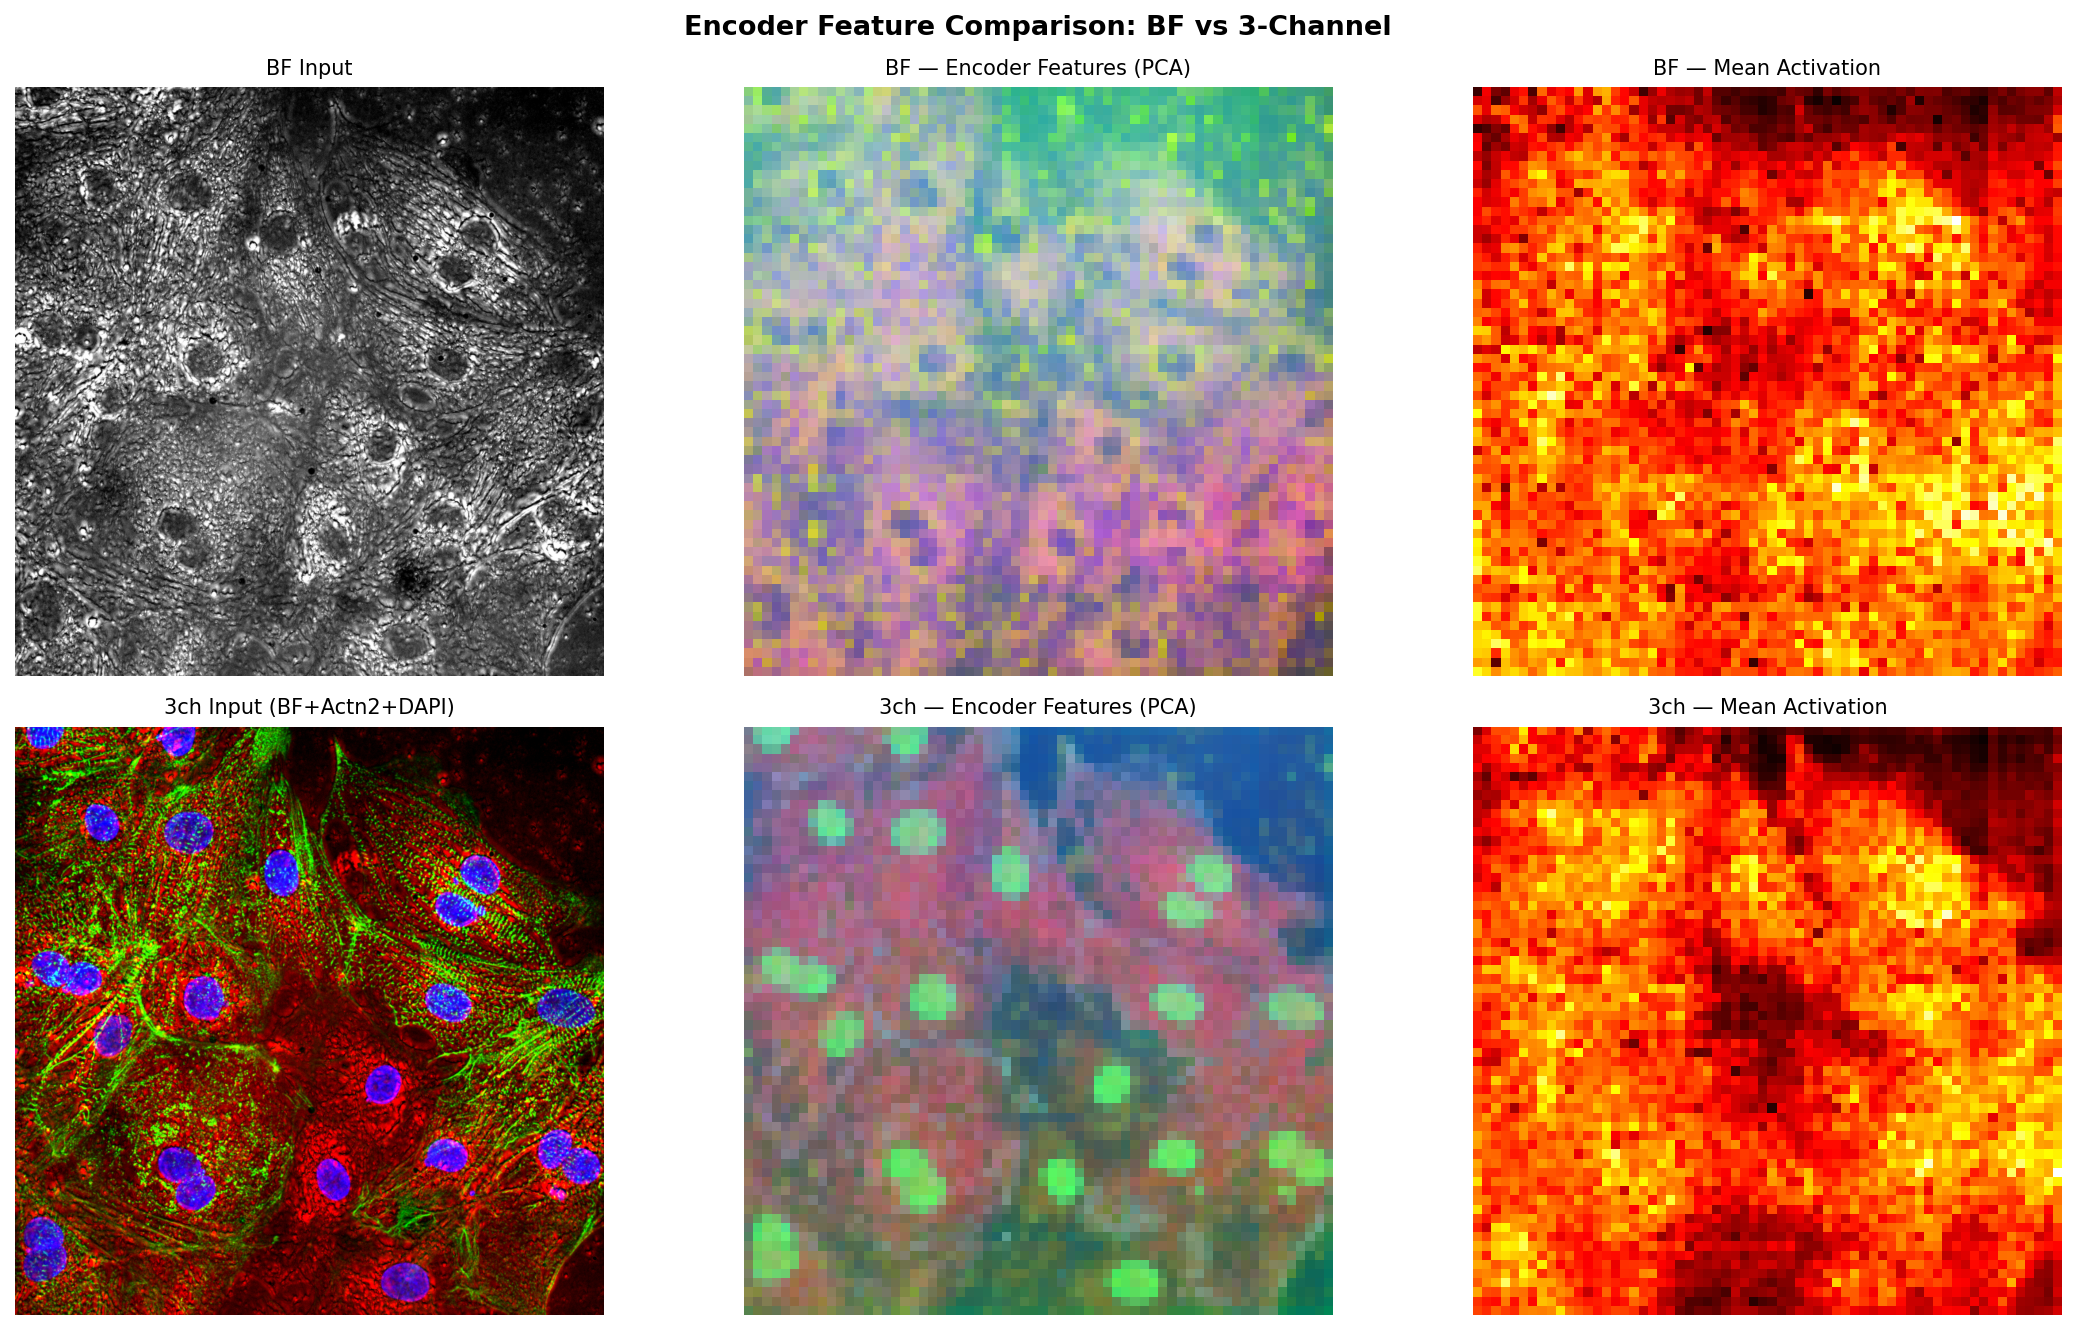
\includegraphics[width=\linewidth]{figures/t28_attention_heatmap_9797a59f_5500000013_63X_20190807_S2_P16_C5.png}
  \caption{T28 encoder activation heatmap under BF-replicate versus three-channel input. This figure provides qualitative representation-level evidence only.}
  \label{fig:app_t28_encoder_heatmap}
\end{figure}

\begin{figure}[t]
  \centering
  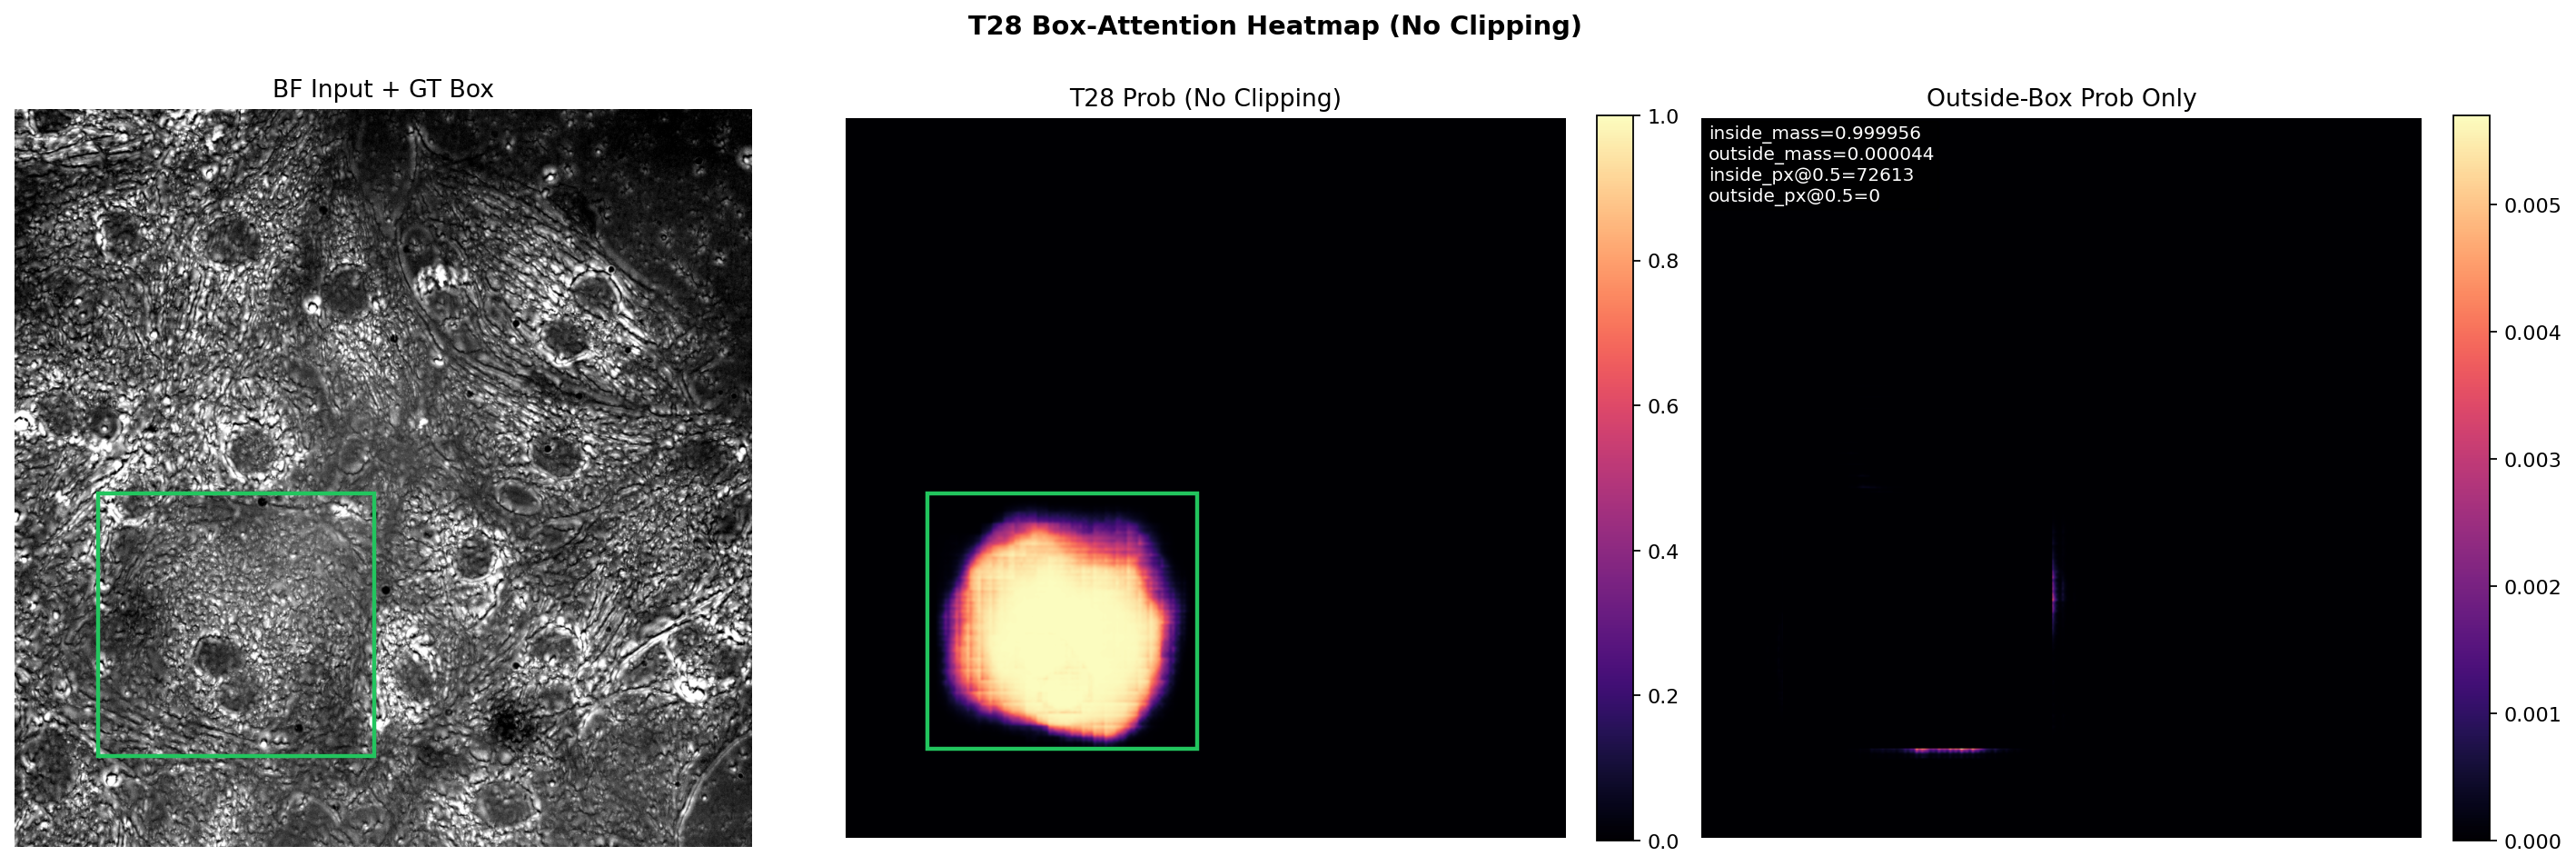
\includegraphics[width=\linewidth]{figures/t28_box_attention_9797a59f_5500000013_63X_20190807_S2_P16_C5_cell10.png}
  \caption{T28 box-outside probability heatmap (no clipping) on one representative sample. The outside-box probability mass is low in this case, which is consistent with weak clipping sensitivity under GT-box settings.}
  \label{fig:app_t28_box_heatmap}
\end{figure}

Both figures are interpreted as sample-level explanatory diagnostics. They should be read together with main-text metrics rather than as independent claims about full-dataset behavior.
